\documentclass{article}

% Language setting
% Replace `english' with e.g. `spanish' to change the document language
\usepackage[english]{babel}

% Set page size and margins
% Replace `letterpaper' with `a4paper' for UK/EU standard size
\usepackage[letterpaper,top=2cm,bottom=2cm,left=3cm,right=3cm,marginparwidth=1.75cm]{geometry}

% Useful packages
\usepackage{amsmath}
\usepackage{graphicx}
\usepackage[colorlinks=true, allcolors=blue]{hyperref}

\title{Robustness Training in Four Procedures of Machine Learning}
\author{Wei Yichen}

\begin{document}
\maketitle

\begin{abstract}
This paper examines the importance of robustness in machine learning, particularly in view of the iterative models and innovative data analysis architectures that have improved the ability to exploit diverse features and uncover complex relationships within datasets. However, a significant portion of the data is often noisy or toxic, requiring robust training techniques. We analyse existing robust training techniques from four key perspectives: input training data, deep neural architecture, regularisation and loss function. In addition, we suggest possible future research directions in this area, and provided an experiment of noise prediction's feasibility to show the potential of the possible future robustness training. The code can be found on \url{https://github.com/OwenCalstroy/Robustness-Training-in-Four-Procedures-of-Machine-Learning}
\end{abstract}

\section{Introduction}

In recent years, the ability to mine datasets has been greatly improved by the development of iterative models in various domains and the emergence of advanced data analysis architectures. These advances enable the exploitation of diverse features and the identification of intricate relationships, ultimately improving the generalisation capabilities of machine learning. However, it is important to recognise that a significant amount of data may contain high levels of noise or even toxic elements. Therefore, ensuring the robustness of the entire machine learning process becomes essential. This paper aims to deepen the understanding of robustness in machine learning by analysing existing robust training techniques from the perspective of the input training data, the deep neural architecture, the regularisation and the loss function, which are all parts involved in the deep learning model training process as shown in Figure 1.

\begin{figure}
\centering
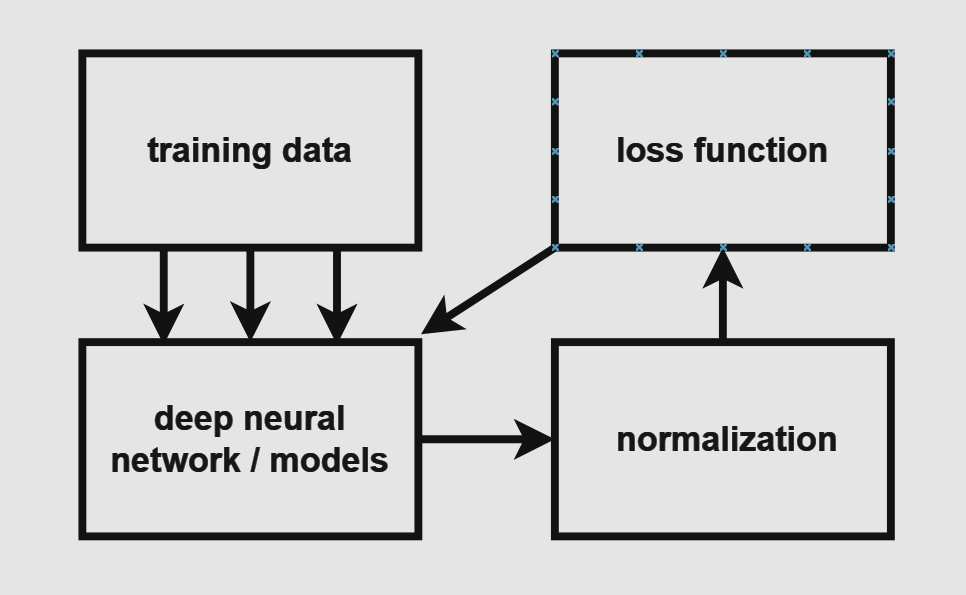
\includegraphics[width=0.75\linewidth]{deep_learning_process_pic.jpeg}
\caption{\label{figure 1:}The deep learning model training process}
\end{figure}

\section{Current robustness training methods}

In the field of machine learning, even the smallest disturbance can affect the final result dramatically. The development of robustness training methods has pushed the whole field to a higher position with higher accuracy and less possibility to be wrongly trained when facing the large amount of data with noises and inaccuracies in the real world. All of the improvement are made in the following four perspectives: input training data, deep neural architecture, regularisation, and loss function, all of which plays an irreplaceable part in the whole process.

\subsection{Input Training Data}

If we want to enhance the robustness of the model when training the deep neural network, organizing and purifying training data in the first place will be the most efficient and easy way. We will discuss this in several aspects.

Enhancing the datasets. There were some classic methods to enhance datasets,: the application of techniques such as panning, rotation, zooming, resolution alteration, colour modification, and others serves to expand the dataset, thereby enhancing the generalisation achieved through training and conferring enhanced resilience to future data. There are also some new techniques, like CutMix\cite{yun2019cutmixregularizationstrategytrain}, achieved by combining two distinct input samples to create a novel training sample, and Cutout\cite{devries2017improvedregularizationconvolutionalneural}, achieved by randomly erasing pixels from a single or multiple sub-regions within the image.

Adding noise into the dataset. The inclusion of random noise in the training data enables the model to become more adaptable to the types of noise that may be present in real-world data\cite{6889193}. \cite{rakin2018parametricnoiseinjectiontrainable}. There are also more recent studies like Structured noise injection\cite{alharbi2020disentangledimagegenerationstructured}, which introduces a spatial noise coding approach, whereby the input tensor is divided into distinct regions, each assigned a unique noise code. Additionally, a separate mapping is established for each code, corresponding to its respective region. This enables the generation of more detailed results. And approach implements additional optimizable weights to inject uncorrelated noise into the existing feed-forward network architecture through the use of Noise Injection Nodes (NINs) \cite{levi2022noiseinjectionprobedeep}. 

Data and category balancing. This includes Batch normalization\cite{ioffe2015batchnormalizationacceleratingdeep}, which serves to reduce internal covariate bias by introducing normalisation operations in each layer of the neural network. It also includes SMOTE\cite{Chawla_2002}, achieved through the combination of oversampling a select number of classes and undersampling the majority class, and many other methods.


\subsection{Deep Neural Architecture}

The primary advancement in deep neural network architecture for improving resilience is adversarial training. In 2014, Christian Szegedy demonstrated that the perturbation of the dataset will result in a completely different training trajectory\cite{szegedy2014intriguingpropertiesneuralnetworks}, highlighting the profound impact of In the same year. In the same year Goodfellow introduced the Fast Gradient Sign method\cite{Goodfellow2014GenerativeAN} , which employed an adversarial process to generate new models with the aid of the backpropagation method. Subsequently, Moosavi-Dezfooli (2016), Carlini and Wagner (2017), Zhang (2019) and Wang (2024) all proposed new models to enhance the model's robustness from large datasets.

Consider that most of the development is oriented from loss function or normalization, I am picking the ones that mainly focus on the model architecture itself in this section.

BIM (basic iterative method) \cite{kurakin2017adversarialmachinelearningscale} generates adversarial samples by repeatedly adding perturbations to the gradient direction, with each step of the perturbation based on the current input gradient information. MIM (momentum-based basic iterative method) \cite{dong2018boostingadversarialattacksmomentum} represents an improvement on BIM. The method draws on the analogue momentum approach, which has been previously introduced in the context of parameter updating in neural networks. In each round of perturbation, the current gradient direction is related to both the gradient direction computed in the previous iteration and the current input gradient.

DeepFool\cite{moosavidezfooli2016deepfoolsimpleaccuratemethod}, introduced by Moosavi-Dezfooli, employs the 'fast gradient sign' approach to identify th-e minimal perturbation that can alter the classifier's decision. Consequently, the performance of the entire structure in response to potential perturbation datasets was evaluated and found to be significantly enhanced. However, this approach is dependent on extensive computational resources, yet it remains inadequate in scenarios that necessitate targeted processing. This is fatal when facing large-scale datasets that the model nowadays receives and also needs to achieve higher quality and accuracy.

AdvXL\cite{wang2024revisitingadversarialtrainingscale}, introduced by Wang, was employed and operated on a large-scale dataset, for over 1 billion samples. the framework depends on a light pre-training stage and an intensive fine-tuning stage. The main idea is to first deploy a long training with weaker attacks and then deploy a short training with harsh attacks, in order to maintain the efficiency while reducing the calculating costs. Moreover, they employ CLIP text encoder to extract classifier weights when dealing with the large-scale datasets (specifically in their research, web-crawled ones). This technique provides a solution for large-scale of data, allowing the model to enter training with a relatively accurate initial state, ultimately producing training results with less deviation and better robustness. This idea solves the large-scale datasets problem, providing a new perspective when confronted with possible poisonous and noisy data. However, recognizing and separating the data for the pre-training stage is still a demanding job, which will lead to more dominant position of poisonous and noisy data in the pre-training stage if not done well, because recognizing the poisonous and noisy data as data with weak attacks will definitely hurt the model at the beginning. If the characteristic of the chosen data is homogeneous and extreme,  the pre-training stage will also provide a biased model, harming the fine-tuning stage.


\subsection{Normalization}

Regularisation is a key step in the machine learning process. It prevents overfitting and enhances the generalisation ability of the model by applying penalties that prevent the parameters from being incorrectly influenced by the data. In addition, if the appropriate regularisation method is chosen, the computational complexity can be reduced on top of the above, resulting in better model training results. The development of regularisation techniques in machine learning demonstrates the importance that researchers place on the robustness of the trained models.

Based on Dropout, Dropblock\cite{ghiasi2018dropblockregularizationmethodconvolutional}, introduced by Golnaz Ghiasi, made a further approach for structured data. It removes entire contiguous regions from the feature map of a given layer, rather than merely deleting individual units at random. The whole process was completed by randomly choosing and then adopting masks onto the input sample before the final normalization process. The method is designed to facilitate the acquisition of spatially distributed representations.  This demonstrates that the specification of normalisation in response to diverse scenarios may yield superior outcomes. Given that each scenario and case may possess disparate value propositions and that the emphasis on varying aspects may result in disparate performance outcomes, this is an important consideration.

Entropy Regularization\cite{han2019unsuperviseddomainadaptationcalibrating}, introduced by Ligong Han, established a method using the idea of Renyi entropy. It enables the model to achieve higher uncertainty when facing ambiguous input, which has higher entropy, while lower when the input is trustworthy, therefore exploring a broader range of predictions. The entropy value is typically obtained by deep neural networks, which generate discrete distributions of potential classes based on the input data. This allows the uncertainty of the prediction to be quantified. This method decreases the complexity and data volume, and is also suitable for a variety of situations. However, it is complex in entropy computation, and may be sensitive to noise, therefore failing to provide a more robust model.

The Information Bottleneck, brought out by \cite{tishby2000informationbottleneckmethod} and introduced into the deep learning field by \cite{shwartzziv2017openingblackboxdeep},  is a method of compressing read data by refining relevant information, thereby reducing the workload while retaining core information. The core objective is "to minimise the complexity of the representation (i.e. compress the data) while maximising information relevant to a specific target variable" \cite{shwartzziv2023compresscompressselfsupervisedlearning}. This approach reduces the impact of noise and erroneous data in multidimensional datasets by maintaining essential information.  Nevertheless, it is inevitable that some valid information will be excluded due to the information bottleneck and causing the suboptimal utilisation of data. However, the reduced computational burden and superior outcomes make it a dependable option.

The Information Bottleneck is part of the Mutual Information Maximization progress. The objective of Mutual Information Maximization is to achieve the greatest possible mutual information between two random variables. There are other similar works like Deep InfoMax\cite{hjelm2019learningdeeprepresentationsmutual},  which "perform unsupervised learning of representations by maximizing mutual information between an input and the output of a deep neural network encoder", and Contrastive Predictive Coding\cite{oord2019representationlearningcontrastivepredictive}, which predict the future in the latent space through robust autoregressive modelling, using probabilistic contrastive loss to capture the information most useful for predicting future samples, etc..

\subsection{Loss Function}

Loss function is an important part in machine learning. It offers a quantitative method to show the distance between the current trained model and the ideal target model. Designing and choosing the proper loss function in different situations will affect greatly how the model performs,  therefore enhancing the robustness of the loss function will improve the accuracy and efficiency of the whole model. Here are some popular optimization in loss function robustness.

Huber loss function\cite{huber2011robust}, introduced by Huber P.J., is an appropriate tool for handling data sets that contain outliers. The Huber loss function combines the advantages of mean square error (MSE) and mean absolute error (MAE) by setting a threshold and using MSE when the value is less than the threshold and MAE when it is equal to or greater than the threshold. This approach allows for a reduction in sensitivity when large errors are encountered and the smoothing of the optimisation process when small errors are present. This results in an improved robustness of the model.

Label smoothing \cite{szegedy2015rethinkinginceptionarchitecturecomputer}, introduced by Christian Szegedy, achieved better robustness by changing the final target from 1 to 1 - LS, where LS is the label smoothing constant. It overcomes the fact that ordinary loss only considers the loss of correct label positions and does not focus on reducing the probability of predicting incorrect labels, reducing the severity of judgemental targets for correct outcomes leads to better prosperity. This is an easy but efficient way to strengthen the robustness of the model during training, but it remains incapable when facing high-precision tasks because it sacrificed detailed accuracy in order to gain high robustness.

GANetic loss \cite{akhmedova2024ganeticlossgenerativeadversarial}, introduced by Shakhnaz Akhmedova, takes a different prospective in loss function optimization. The method employs genetic programming to identify the optimal loss function, conceptualising the loss function as the objective of an optimization process. In the process of loss function optimisation, parameters are randomly selected from $\{y_{pred}, y_{real}, real\ numbers\}$, and the operator from \{plus,minus,multiply,divide,square root,log,exp,sin,cos\} , to form a loss function format. Subsequently, genetic programming is employed to iteratively refine the relatively effective loss functions, ultimately identifying a robust function with broad applicability across diverse datasets. This approach effectively addresses the challenge of designing effective loss functions and has yielded promising outcomes. Moreover, it has paved the way for the development of a universal, robust loss function that enhances model performance across different data types, offering insights into the design of loss functions in general. Nevertheless, the quality of the initial training datasets is of the utmost importance, requiring minimal error data and the most efficient type to achieve a more general loss function, which is a costly process.

Another interesting study is MCGAN \cite{xiao2024mcganenhancinggantraining}, which introduced a new regression loss into GAN, integrating Monte Carlo method into data sampling, and successfully solve the training instability. Therefore, it is suggested that integrating existing algorithms and methods in the classic computer science field, or simulating and analogizing studies and theories (like physics) in deep learning methods, may receive terrific results.

Free adversarial training, introduced by Ali Shafahi, reuses the backward pass for the next training process for the same mini batch, creating a closer relationship between the input and optimization. Through repeatedly using the same mini batch, this method reduces the requirement of high computational power, and can achieve higher robustness while demanding little additional cost. This work was efficient on small-scale datasets and saving computational power, but did not actually solve the fundamental robustness problem in situations with large-scale datasets and enough computational power (ideally). This means that such method requires further optimization or complete change.



\section{Predictions and Outlooks towards Robustness Training and Enhancement}

The field of model robustness is experiencing a surge in research activity, with an increasing number of researchers engaged in efforts to mitigate the impact of noise and enhance model generalisation and robustness. In light of the aforementioned findings, I presents the following predictions and outlook for future research in the field of robustness training.

Firstly, it is essential to consider the integration of established methodologies. At present, the majority of methodologies lack robustness in diverse scenarios. This is evident in specific domains such as image processing and large language modelling, where they are either not applicable or unable to focus on the distinct aspects emphasised in different domains (For instance, proximity interrelationships in image processing and word and paragraph order correlations in large language modelling). The novel approaches may potentially facilitate the extraction of similarities from the disparate emphases inherent to disparate domains (e.g., when dealing with a single sample, to generalise the order of elements within the single sample, the relative distance relationship, etc.). Furthermore, it may enable the identification of a more general approach that can simultaneously address the core concerns of disparate domains.

Secondly, the introduction of additional models and concepts from subject areas such as physics, chemistry, biology, traditional computer science, and so forth, will facilitate more innovative modelling of noisy, harmful, and normal data, thereby achieving new results. As previously demonstrated with genetic algorithms, simulated annealing algorithms, and so forth, the combination of analogues of existing models from disciplines such as physics and chemistry with robustness training may yield superior and less arithmetic-demanding results in certain instances.

Thirdly, the prediction of noise may also prove to be a significant advancement in the field of machine learning, particularly in terms of enhancing the robustness of such models. This may rely especially on machine learning to recognize the 'noise pattern' and then producing the most suitable model. It can be postulated that noise in reality will also exhibit certain patterns. Researchers can identify and model noise in data with the assistance of machine learning, thereby forming reasonable noise estimates for specific datasets. This enables the identification of potential outlier noise points as well as malicious data. Learning noise as a normal retained part of the data rather than removing it may yield enhanced robustness and generalisation. It would be beneficial to explore whether this direction can be developed with mutual reference to chaos in physics research.

Fourthly, the combination of robust training and computer security represents a potential avenue for future development. Robust training can be conceptualised as a form of data security, serving to safeguard against the detrimental impact of malicious data as well as the overfitting outcomes associated with an excessively low probability of 'perfect' data. Consequently, it would be fruitful to draw upon pertinent experiences and models from the domain of computer security and adapt them to the context of machine learning.

It can be stated that robustness training for machine learning still has significant room for improvement. Future research will concentrate on enhancing the adaptability and stability of models in complex, dynamic environments with large data volumes, particularly in domains such as combating attacks, data noise, and responding to real-world changes. It seems probable that the future development of robust training methods will be informed by the introduction of deep learning (as exemplified by  \cite{akhmedova2024ganeticlossgenerativeadversarial}). This approach is likely to complement the development of machine learning models, with the goal of achieving even better results.


\section{Experiment}

For the third point, which is learning the noise pattern with machine learning, and then predicting the noise, I give out such experiment to justify the huge advantage it will bring to the whole training process, enhancing the robustness of the model and boosting the efficiency of the learning process.

Let us suppose that the natural data exhibit a pattern of normal distribution with respect to the noise. If we can successfully learn that:

\begin{enumerate}
    \item The noise pattern of the input data exhibits characteristics similar to a normal distribution.
    \item The approximate mean and standard deviation can be calculated.
\end{enumerate}

Then we can greatly increase the efficiency of the training process and the robustness of the model.

In this simulation, it is hypothesised that the prediction will be realised through the application of machine learning. A normal distribution was added to the idealised dataset in order to simulate the natural noise. Two training processes were then conducted: one with the dataset before the predicted noise pattern was removed, and the other with the dataset after the predicted noise pattern was removed. The results demonstrate that the latter process exhibits a consistently diminishing loss number in every epoch, thereby progressing towards the target function (represented by the equation $y = 2.1 + 3.2x + 1.6x^2 + 0.9x^3$ in this experimental simulation) at an accelerated rate. Such result remains the same for different means and standard deviation, as is shown in Figure 2, Figure 3, Figure 4, Figure 5. The code website can be found in the abstract.

\begin{figure}
\centering
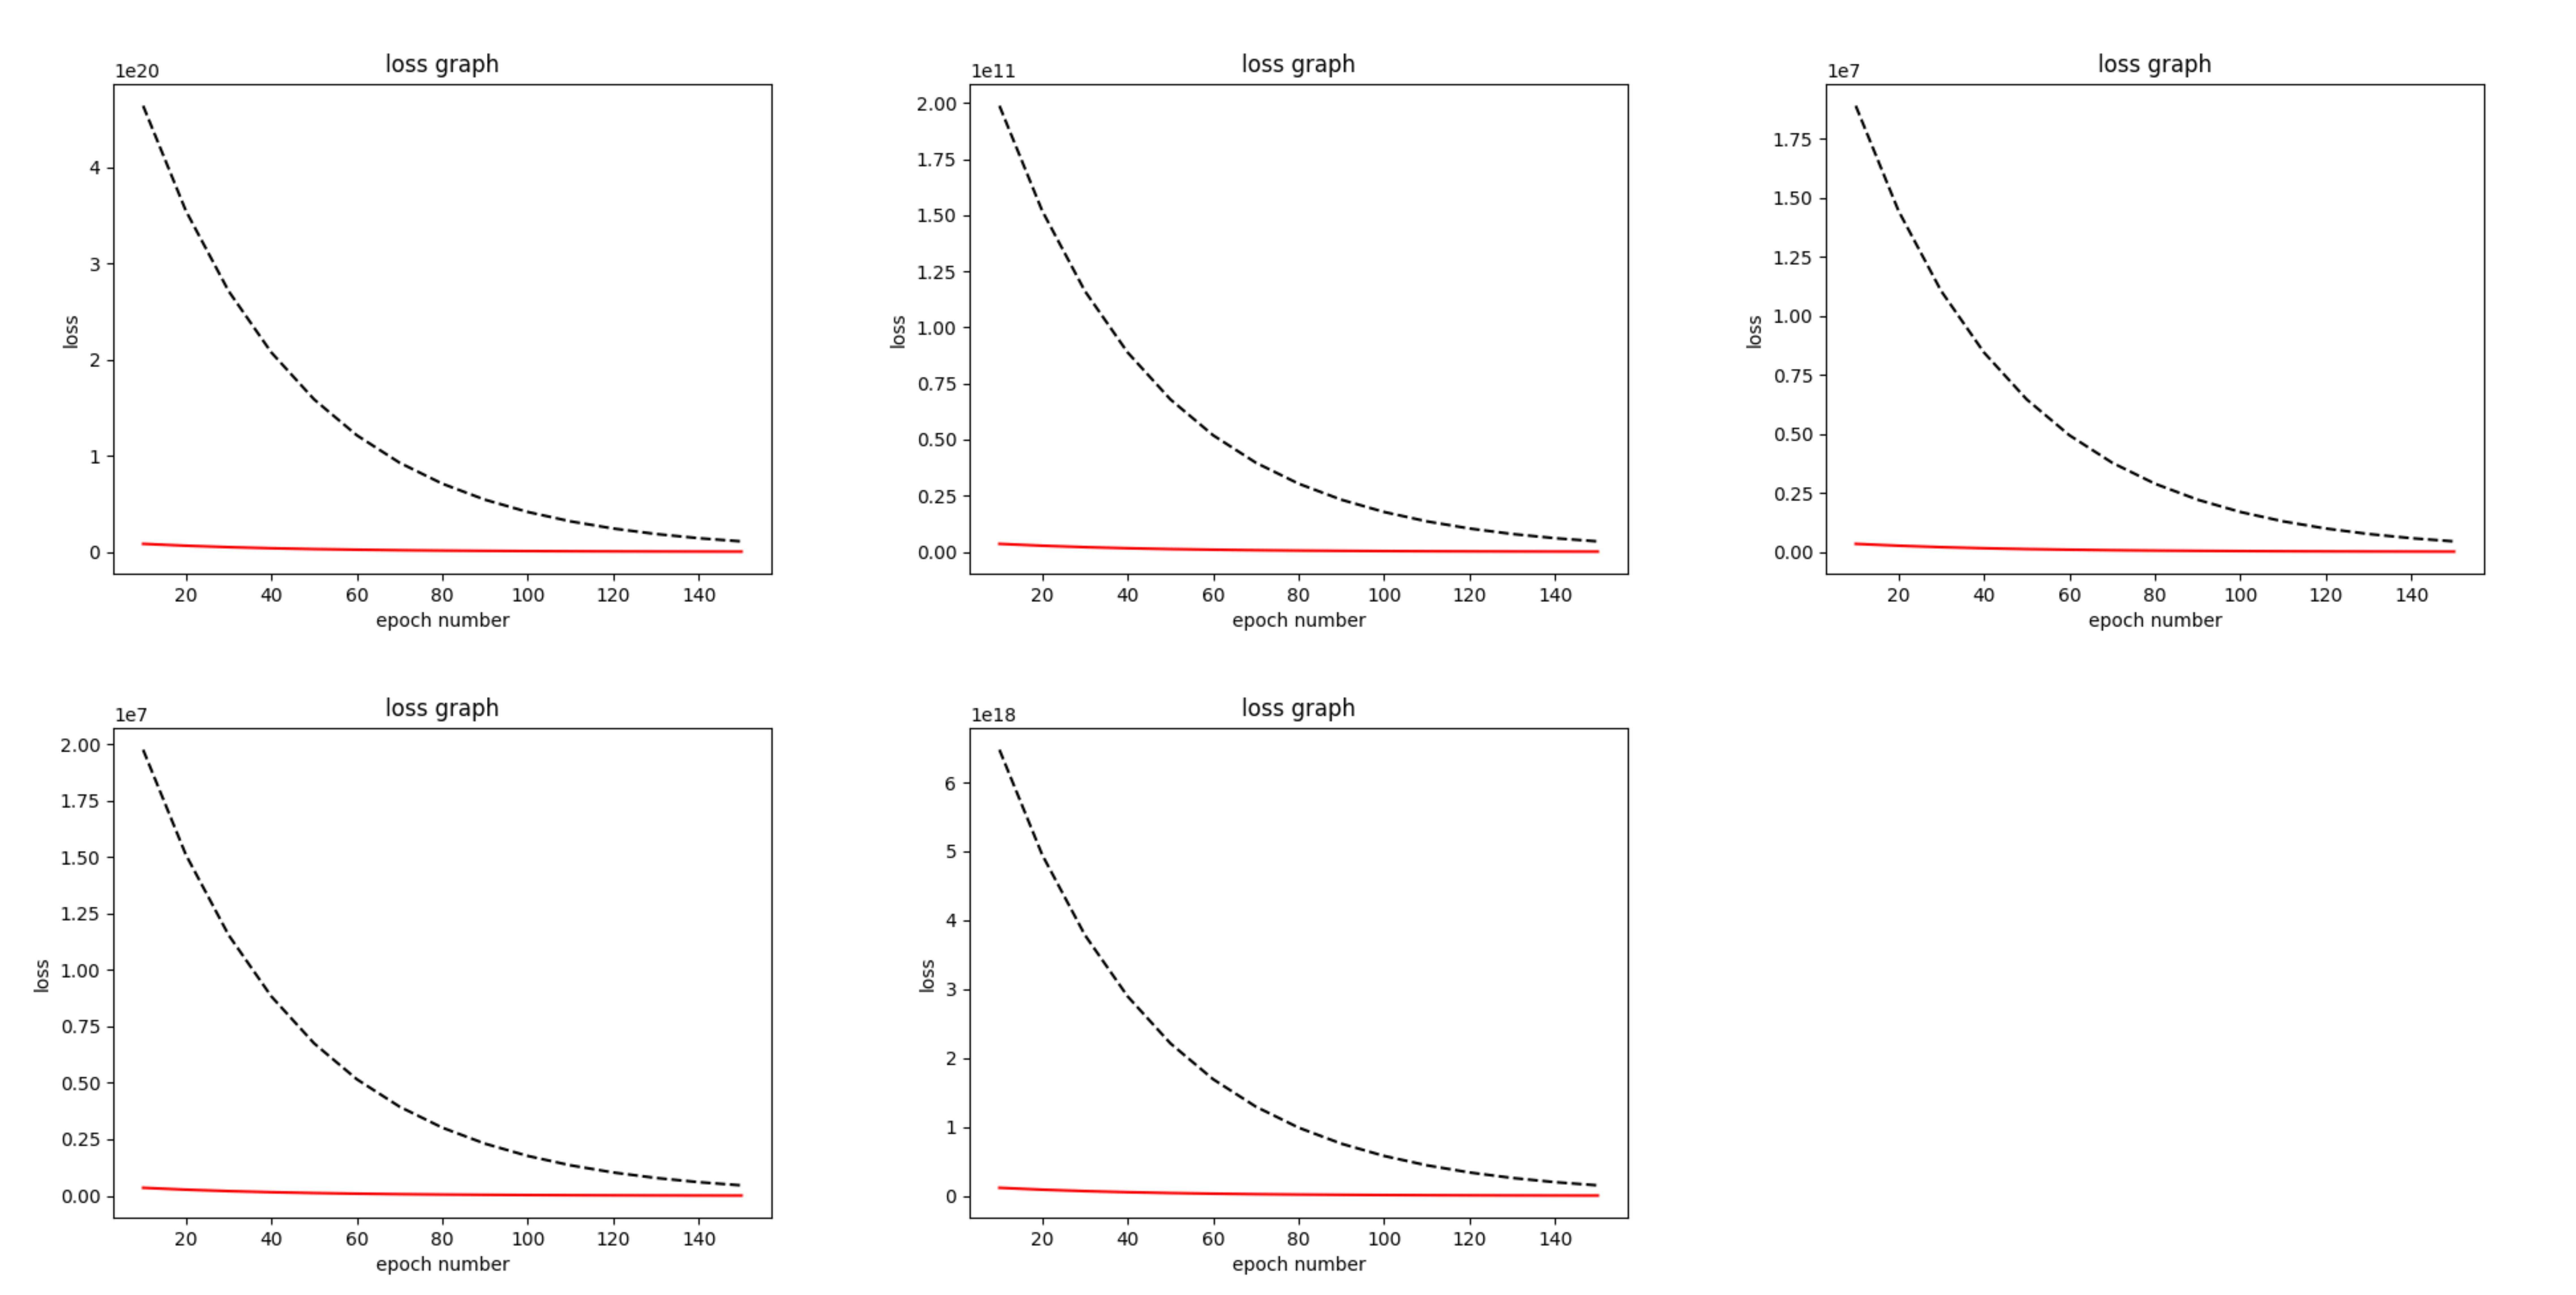
\includegraphics[width=0.75\linewidth]{Fig(0.0,0.1).jpg}
\caption{\label{figure 2:}$(mean, \sigma) = (0.0, 0.1)$ and simulating learned parameters $(mean, \sigma) = (0.01, 0.08)$}
\end{figure}

\begin{figure}
\centering
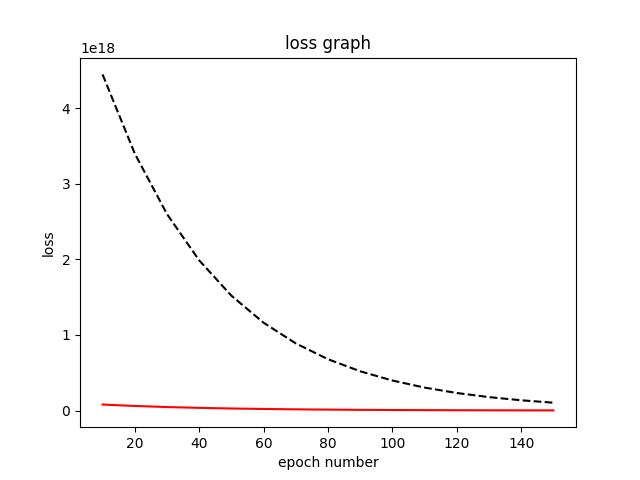
\includegraphics[width=0.5\linewidth]{Fig(0.0,0.5).png}
\caption{\label{figure 3:}$(mean, \sigma) = (0.0, 0.5)$ and simulating learned parameters $(mean, \sigma) = (0.2, 0.48)$}
\end{figure}

\begin{figure}
\centering
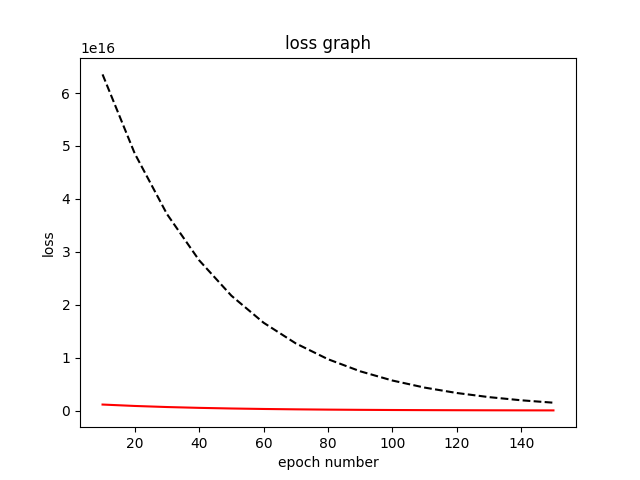
\includegraphics[width=0.5\linewidth]{Fig(0.0, 1.0).png}
\caption{\label{figure 4:}$(mean, \sigma) = (0.0, 1.0)$ and simulating learned parameters $(mean, \sigma) = (0.1, 0.9)$}
\end{figure}

\begin{figure}
\centering
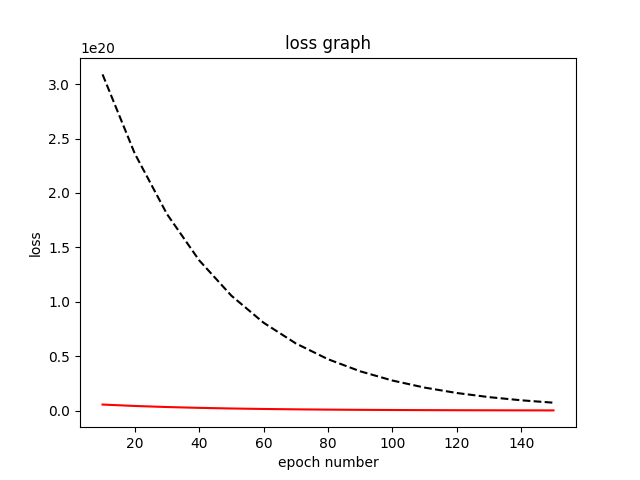
\includegraphics[width=0.5\linewidth]{Fig(3.0,1.0).png}
\caption{\label{figure 5:}$(mean, \sigma) = (3.0, 1.0)$ and simulating learned parameters $(mean, \sigma) = (2.8, 0.9)$}
\end{figure}
In this experiment, it is shown how powerful it will be if the machine can learn the pattern of the noise, and then extract the 'purified ideal' dataset from the natural dataset with noise. Therefore, there remains to be a lot of further exploration in the field of robustness training in different procedures of machine learning, making it a promising and useful field for future researchers to dive in.

\subsection{Conclusion}

In this paper, we analyse existing robust training techniques from four key perspectives: input training data, deep neural architecture, regularisation and loss function, realizing that there have been plenty of useful and profound measures in different perspectives. Moreover, we suggest possible future developing directions in this area, and provided an experiment of noise prediction's feasibility to show the potential of the possible future robustness training. This experiment shows the enormous potential of noise prediction, which demonstrate that the robustness training is still in its infancy and a considerable amount of time will elapse before it reaches a point of maturity.



\bibliographystyle{unsrt}
\bibliography{sample}

\end{document}
